\documentclass[10 pt]{article}
\usepackage{tikz}
\usetikzlibrary{arrows}
\usepackage[margin=0.5 in]{geometry}
\usepackage[utf8]{inputenc}
\usepackage{tabu}
\usepackage{color}
\usepackage{xcolor}
\usepackage{listings}
\usepackage{enumitem}
\usepackage{multicol}
\setlength{\columnsep}{1cm} 
\title{\textbf {Estructuras de Datos 1 - ST0245\\Segundo Parcial Grupo 033 (Lunes)}}
\author{Nombre ..............................\\
		Departamento de Informática y Sistemas\\
		Universidad EAFIT\\}
\date{Mayo 7 de 2018}
\begin{document}
\lstdefinestyle{customc}{
	language=Java, 
	numbers=left, 
	showspaces=false,
    showstringspaces=false, 
    tabsize=2, 
    breaklines=true,
    xleftmargin=5.0ex,
}
\lstset{escapechar=@,style=customc, numbers=left, stepnumber = 1} 
\maketitle
\begin{multicols}{2}
Para propósitos de este parcial se considerarán las siguientes implementaciones de  árbol binario y árbol n-ario.
\begin{lstlisting}
//Arbol binario
class BNode{
  BNode izq;
  BNode der;
  int val;
}
//Arbol n-ario
class NNode{
  ArrayList<NNode> hijos;
  int val;
}
\end{lstlisting}
\section{Árboles 40\%}
Considere un árbol n-ario cuyos nodos están enumerados de $0$ hasta $n - 1$ y su raíz es el nodo $0$. Como
un ejemplo, este un árbol n-ario donde $n=15$.
\\
\begin{center}
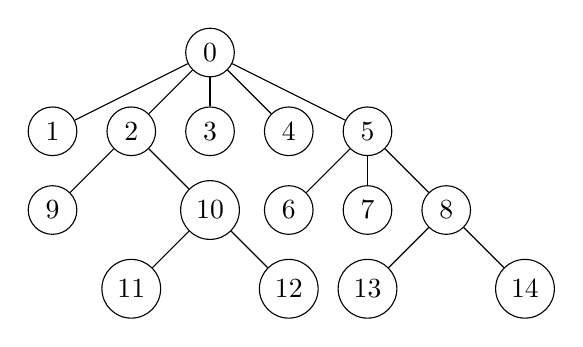
\begin{tikzpicture}

\tikzset{vertex/.style = {shape=circle,draw,minimum size=1.5em}}
\tikzset{edge/.style = {-,> = latex'}}
\node[vertex] (0) at (0,1)  {0};
\node[vertex] (1) at (-2,0)  {1};
\node[vertex] (2) at (-1, 0) {2};
\node[vertex] (9) at (-2, -1) {9};
\node[vertex] (10) at (0, -1) {10};
\node[vertex] (11) at (-1, -2) {11};
\node[vertex] (12) at (1, -2) {12};
\node[vertex] (3) at (0, 0) {3};
\node[vertex] (4) at (1, 0) {4};
\node[vertex] (5) at (2, 0) {5};
\node[vertex] (6) at (1, -1) {6};
\node[vertex] (7) at (2, -1) {7};
\node[vertex] (8) at (3, -1) {8};
\node[vertex] (13) at (2, -2) {13};
\node[vertex] (14) at (4, -2) {14};

%edges
\draw[edge] (0) to (1);
\draw[edge] (0) to (2);
\draw[edge] (0) to (3);
\draw[edge] (0) to (4);
\draw[edge] (0) to (5);
\draw[edge] (5) to (6);
\draw[edge] (5) to (7);
\draw[edge] (5) to (8);
\draw[edge] (2) to (9);
\draw[edge] (2) to (10);
\draw[edge] (10) to (11);
\draw[edge] (10) to (12);
\draw[edge] (8) to (13);
\draw[edge] (8) to (14);
\end{tikzpicture}
\end{center}

Para un \textbf{sub-árbol} cuyo nodo raíz es el nodo $u$, el \textbf{tamaño} del sub-árbol $u$, denotado como $tam(u)$, es la cantidad de nodos que éste contiene; particularmente, $tam(0) = n$. Queremos determinar cuantos nodos contiene cada sub-árbol de nuestro árbol n-ario. Ayúdanos a completar las siguientes líneas.

\begin{lstlisting}
void calcular(int[] tam, 
                    NNodo nodo){
  tam[.............] = 1;
  int hijos = nodo.hijos.size();  
  for(int i = 0; i < hijos; i++){
    int siguiente = nodo.get(i).val;    
      calcular(tam, siguiente);
      tam[........] += tam[nodo.val];      
    }  
  }
}
int[] calcular(int n, NNodo raiz){  
  int[] tam = new int[..........];
  calcular(tam, raiz);
  return tam;
}
\end{lstlisting}
\begin{enumerate}[label=\alph*]
\item (10\%) Completa la línea 3  .............
\item (10\%) Completa la línea 8 .............
\item (10\%) Completa la línea 13 .............
\item (10\%) ¿El árbol anterior es un \textbf{\textit{árbol binario de búsqueda}}?
\begin{enumerate}[label=(\roman*)]
\item Verdadero
\item Falso
\end{enumerate}
\end{enumerate}
\section{Pilas 20\%}
El método \texttt{push(i)} ingresa el elemento $i$ al tope de la pila. El método \texttt{pop()} retira
el elemento en el tope de la pila y retorna su valor. Considere el siguiente método:
\begin{lstlisting}
void metodo(Stack<Integer> s){
  for(int i = 10; i >= 0; i--){
    if(i % 2 == 0){
      s.push(i);    
    }  
  }
  System.out.print(s.pop());
  while(s.size() > 0){
    System.out.print(" " + s.pop());  
  }
}
\end{lstlisting}
\begin{enumerate}[label=\alph*]
\item (10\%) ¿Cuál es la salida del método anterior?
\begin{enumerate}[label=(\roman*)]
\item 10, 8, 6, 5, 4, 2, 0
\item 2, 4, 6, 8, 10
\item 1, 2, 3, 4, 5, 6, 7, 8, 9, 10
\item 0, 2, 4, 6, 8, 10
\end{enumerate}
\item (10\%) ¿Cuál es la complejidad asintótica, en el peor de los casos, de añadir un nuevo elemento a una pila que contiene $n$ elementos?
\begin{enumerate}[label=(\roman*)]
\item $O(1)$
\item $O(n)$
\item $O(n \log n)$
\item $o(n^2)$
\end{enumerate}
\end{enumerate}
\section{Colas 20\%}
El método \texttt{add(i)} agrega el elemento $i$ al inicio de la cola. El método \texttt{poll()} retira el elemento al final de la cola y retorna su valor. Considere el siguiente método:
\begin{lstlisting}
void metodo(Queue<Integer> q){
  for(int i = 2; i * i <= 25; i++){
    q.add(i);  
  }
  System.out.print(q.poll());
  while(q.size() > 0){
    System.out.print(" " + q.poll());
  }
}
\end{lstlisting}
\begin{enumerate}[label=\alph*]
\item (10\%) ¿Cuál es la salida del algoritmo anterior?
\begin{enumerate}[label=(\roman*)]
\item Los enteros positivos menores que 26 en orden ascendente.
\item Los enteros positivos menores que 26 en orden descendente.
\item 2, 3, 4, 5
\item 5, 4, 3, 2
\end{enumerate}
\item (10\%) ¿Cuál es la complejidad asintótica, en el peor de los casos, de retirar un elemento de una cola que contiene $n$ elementos?
\begin{enumerate}[label=(\roman*)]
\item $O(1)$
\item $O(\log n)$
\item $O(n)$
\item $O(n \log n)$
\end{enumerate}
\end{enumerate}
\section{Grafos 20\%}
Considera el siguiente grafo:
\\
\begin{center}
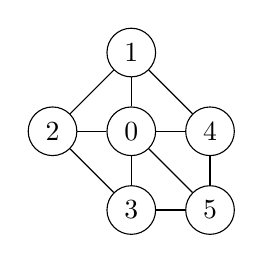
\begin{tikzpicture}

\tikzset{vertex/.style = {shape=circle,draw,minimum size=1.5em}}
\tikzset{edge/.style = {-,> = latex'}}
\node[vertex] (0) at (0,1)  {0};
\node[vertex] (1) at (0,2)  {1};
\node[vertex] (2) at (-1, 1) {2};
\node[vertex] (3) at (0, 0) {3};
\node[vertex] (4) at (1, 1) {4};
\node[vertex] (5) at (1, 0) {5};

%edges
\draw[edge] (0) to (1);
\draw[edge] (0) to (2);
\draw[edge] (0) to (3);
\draw[edge] (0) to (4);
\draw[edge] (0) to (5);
\draw[edge] (1) to (2);
\draw[edge] (2) to (3);
\draw[edge] (3) to (5);
\draw[edge] (5) to (4);
\draw[edge] (4) to (1);
\end{tikzpicture}
\end{center}

\begin{enumerate}[label=\alph*]
\item (10\%) Completa su representación utilizando listas de adyacencia:
\\
\textbf{Pista: La pregunta NO es calcular la clausura transitiva del grafo, sino la
lista de las adyacencias, es decir, la lista de los vecinos.}
\\
$0 \rightarrow [1 \rightarrow 2 \rightarrow 3 \rightarrow 4 \rightarrow 5]$
\\
$1 \rightarrow$
\\
$2 \rightarrow$
\\
$3 \rightarrow$
\\
$4 \rightarrow$
\\
$5 \rightarrow$
\item (10\%) ¿Cuál es la complejidad asintótica, en el peor de los casos, de determinar si dos vértices están unidos por una arista en la representación de un grafo en \textbf{matrices de adyacencia}?
\begin{enumerate}[label=(\roman*)]
\item $O(1)$
\item $O(n)$
\item $O(n^2)$
\item $O(\log n)$
\end{enumerate}
\end{enumerate}
\end{multicols}

\end{document}